\section {Interactions}
\label{sec:related_work_interactions}
Tasks like removing unwanted points, selecting regions of interest, or creating new geometry are examples of interactions that can be performed on point clouds to improve the data quality of the point cloud and create more distinct visual representations of the objects in the point cloud.  
\\
Demir et al. \cite{demir2015procedural} present a framework for semi-automatic point-cloud segmentation and procedural modeling. Interactive editing tools let the user create new point clouds using procedural copy and paste operations, as well as smart resizing. 
\\
\\
O-Snap by Arikan et al. \cite{arikan-2013-osn} utilizes Schnabel's algorithm to extract an initial model from a point cloud used in a reconstruction and modeling pipeline. Local adjacency relations of the obtained shapes are used in an interactive workflow to snap polygon elements together, while simultaneously fitting the input point cloud to ensure the planarity of the polygons. 
\\
\\
The lasso interaction is a common tool to select regions in the two-dimensional screen space. Yu et al. \cite{yu2012efficient} presents two new methods of interaction using only two-dimensional input. The result are two techniques that turn a two-dimensional lasso into a three-dimensional volume that is fitted to the spatial structure of the point cloud. Similar to sketch-based modeling \cite{igarashi2007teddy}, TeddySelection inflates a user-drawn lasso using a heuristic that takes the local point density into account and fits it to the indented region. CloudLasso uses the Marching Cubes algorithm \cite{lorensen1987marching} to identify and select regions within the lasso where the density is beyond a threshold. Both techniques only use two degrees of freedom, thus can be used in a traditional mouse-based interaction, as well as in direct-touch environments. 

\begin{figure}[ht]
    \centering
    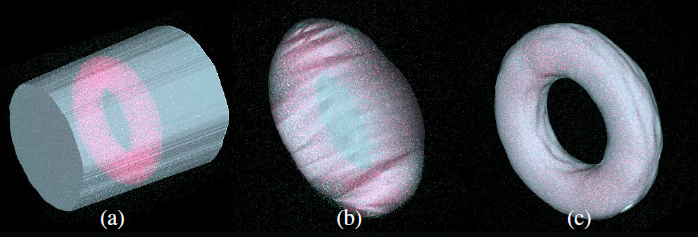
\includegraphics[width=0.81\textwidth]{Related_Work/teddyCloudSelection.png}%7
    \caption[Comparison of (a) simple lasso selection, (b) TeddySelection and (c) CloudLasso]
		{The region in grey describes the selection volume. Points that are selected are colored in pink. (a) shows a simple lasso selection, (b) TeddySelection and (c) shows the CloudLasso. Image by Yu et al.\cite{yu2012efficient}.}
    \label{fig:teddyCloudSelection}
\end{figure}

Figure \ref{fig:teddyCloudSelection} compares the results of a simple lasso selection, TeddySelection and the CloudLasso. 

\par

An example of a three-dimensional interaction technique is the Volumetric Brush by Weyrich et al. \cite{weyrich2004post}. The brush follows the local curvature by retrieving the current depth value for the cursor's position from the zBuffer. The reconstructed world space position is then used to as the center of a volume, usually a sphere, to select points. 

\par

Scheibelbauer and Wimmer \cite{scheiblauer2011out} present an out-of-core point cloud editing system. The system allows for interactive selection and modification of arbitrary parts of a point clouds using a so-called selection octree. This structure is a tool that allows to interactively change the visualization model without actually having to permanently modify the original model. 
